\chapter{Sztuczna inteligencja}
Słownik \textit{Oxford English Dictionary} słowo ,,\textbf{inteligencja}'' definiuje jako zdolność do rozumienia, analizy i dostosowania się do zmian~\cite{OxfordJuly2023}.\ Rozwój nauki i komputerów umożliwił badania nad tworem zbliżonym do możliwości ludzkiej inteligencji, czyli nad sztuczną inteligencją (\textit{ang. Artificial Intelligence, AI}). W ostatnich latach AI dynamicznie się rozwija, znalazła zastosowanie w medycynie, finansach czy w badaniach naukowych.\ Wykorzystywana jest niemal na każdym etapie procesu badawczego: stawiania hipotez, budowania twierdzeń matematycznych, tworzenia i monitorowania badań, zbierania danych czy w wielu innych czynnościach~\cite{AiScience, Mahesh2018}.\ Wśród obszarów sztucznej inteligencji możemy wydzielić m.in. uczenie maszynowe, sieci neuronowe czy uczenie głębokie.\ \refsource{Rysunek}{fig:si-schema} pokazuje rosnącące zawężenie zagadnienia związanego z AI, gdzie uczenie głębokie jest najściślejszym a sztuczna inteligencja najszerszym.

\begin{figure}[H]
    \centering
    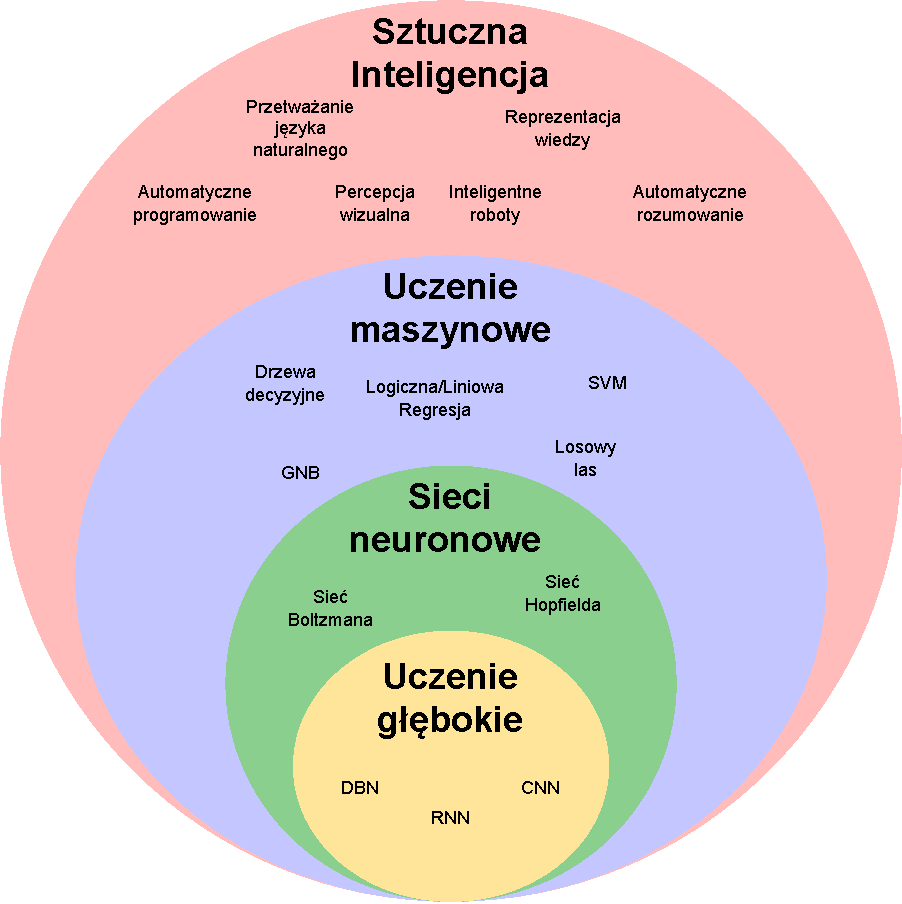
\includegraphics[width=0.5\textwidth]{images/si}
    \captionsource{Graficzne przedstawienie podziałów sztucznej inteligencji}{\cite{LinkedInSi}}
    \label{fig:si-schema}
\end{figure}


\section{Uczenie maszynowe}
Uczenie maszynowe (\textit {ang. Machine Learning, ML}) to dziedzina nauki nad algorytmami oraz modelami statystycznymi, które pracują na dużych zbiorach danych, ucząc się je klasyfikować .\ Algorytmy ML wykorzystuje się m.in. w analizie danych, tworzeniu modeli predykcyjnych, rozpoznawaniu zdjęć czy mowy.\ Dodatkowo nie są zaprogramowane specyficznie pod konkretne zadanie, a jedynie pod grupę zadań.\ Uczenie maszynowe można podzielić na 3 typy, do których należą uczenie: nadzorowane, nienadzorowane oraz ze wzmocnieniem.\ Podział  pokazano na \refsource{rysunku}{fig:ml-schema}.\ Wykorzystanie konkretnego typu uczenia determinuje typ zadania, jaki ma być rozwiązany~\cite{Mahesh2018, LinkedInSi}.

\begin{figure}[H]
    \centering
    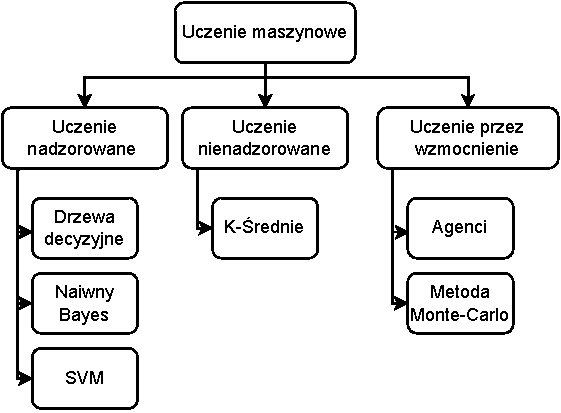
\includegraphics[width=0.6\textwidth]{images/ml-przyklady}
    \captionsource{Podział uczenia maszynowego}{\cite{Mahesh2018}}
    \label{fig:ml-schema}
\end{figure}

\subsection{Uczenie nienadzorowane}
W przypadku uczenia nienadzorowanego algorytm ma sam znaleźć czy występują jakieś wzorce. W porównaniu do uczenia nadzorowanego, tu nie stosuje się zbioru oznaczonego.\ Metodę wykorzystuje się w pracy z danymi, których nie da się zdefiniować np. przy detekcji anomalii, szukaniu wzorców. Pozwala to m.in. na segmentację grup czy wykrywanie anormalnych zachowań np zwiększonego zużycia prądu spowodowanego uszkodzeniem urządzenia elektrycznego.\ Wśród algorytmów uczenia nienadzorowanego wyróżniamy dwie główne metody: K-średnie, klasteryzacja.\ Schemat uczenia nienadzorowanego poprzez klasteryzację jest pokazany na \refsource{rysunku}{fig:unspervised}~\cite{AiScience, Mahesh2018}.

\begin{figure}[H]
    \centering
    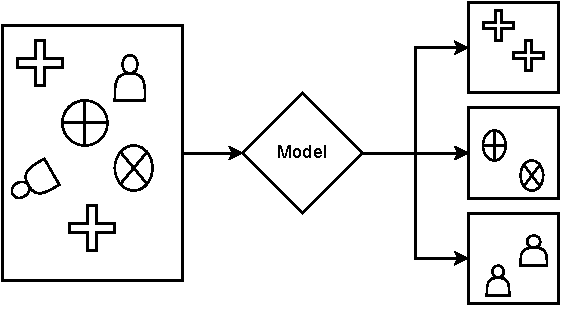
\includegraphics[width=0.5\textwidth]{images/unsupervised}
    \captionsource{Uczenie nienadzorowane}{Opracowanie własne}
    \label{fig:unspervised}
\end{figure}


\subsection{Uczenie nadzorowane}
W procesie uczenia nadzorowanego stosuje się zbiór posiadający etykiety.\ Model uczy się przyporządkowywać określone cechy do konkretnych kategorii.\ Dane wejściowe dzielone są na dane treningowe i dane testowe.\ Zbiór treningowy jest wykorzystywany do trenowania modelu, a zbiór testowy do sprawdzenia rezultatu.\ W trakcie trenowania występuje regulacja modelu.\ Model uczenia został przedstawiony na \refsource{rysunku}{fig:spervised}~\cite{AiScience, Mahesh2018}.

\begin{figure}[H]
    \centering
    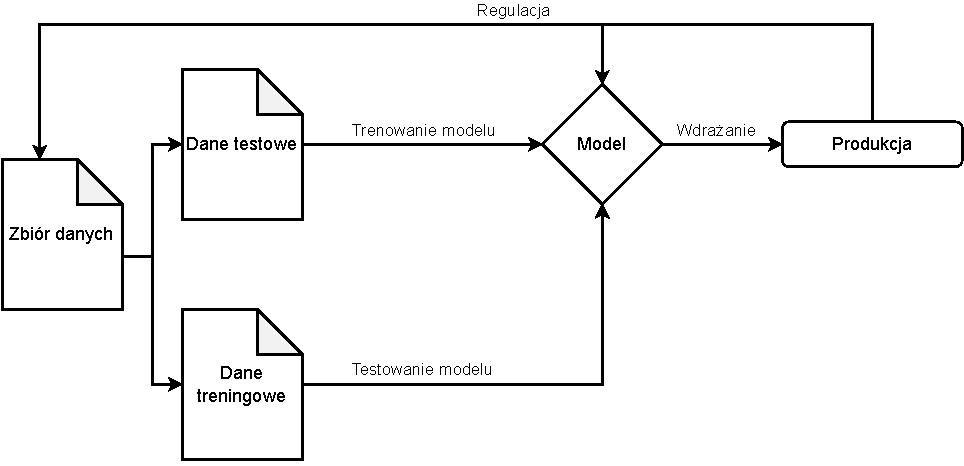
\includegraphics[width=0.8\textwidth]{images/supervised}
    \captionsource{Uczenie nadzorowane}{\cite{Mahesh2018}}
    \label{fig:spervised}
\end{figure}

Algorytmy uczenia nadzorowanego można zastosować między innymi do weryfikacji ruchu sieciowego w celu określenia czy ruch bezpieczny, przez co można to zastosować w systemach wykrywania intruzów (\textit{ang. Intrusion Detection System, IDS}).\ Algorytmy wchodzące w skład uczenia nadzorowanego to m.in. klasyfikator Naiwny Bayesa, drzewo decyzyjne, maszyna wektorów nośnych~\cite{AiScience, Mahesh2018}.

\subsection{Uczenie częściowo nadzorowane}
Jednym ze szczególnych przypadków połączenia uczenia nadzorowanego i nienadzorowanego jest uczenie częściowo nadzorowane.\ Wykorzystywane jest w sytuacjach, kiedy istnieje zbyt duży zbiór danych, którego oznaczenie wiązałoby się z zbyt dużymi kosztami czasowymi i finansowymi.\ Wtedy etykietyzowana jest mała próbka danych, która służy do utworzenia modelu.\ Na podstawie takiego modelu oznacza się pozostały zbiór danych.\ Takie rozwiązanie stosuje się m.in. w bankowości, klasyfikowaniu stron internetowych poprzez wyszukiwanie treści na stronie i kategoryzowaniu ich oraz wyznaczaniu trasy GPS~\cite{semiLinkedin, Mahesh2018}.

\subsection{Uczenie przez wzmocnienie}
Uczenie przez wzmocnienie jest najbliższe ludzkiemu uczeniu się.\ Zbliżona jest do metody ,,\textit{kija i marchewki}''.\ To jest uczenie poprzez nagradzanie dobrych rozwiązań, a karanie złych.\ W odróżnieniu od pozostałych metod uczenia maszynowego, w uczeniu przez wzmocnienie nacisk kładziony jest na przygotowanie odpowiedniego środowiska.\ Jako środowisko określa się zadania lub symulacje, z którymi agent wchodzi w interakcję. Schemat działania przedstawono na \refsource{rysunku}{fig:reinforcemenet}. W tym typie uczenia nie są ważne dane, a rezultat.

\begin{figure}[H]
    \centering
    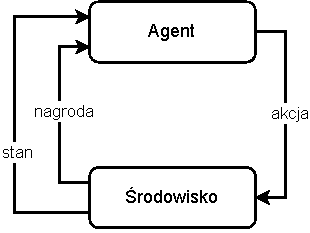
\includegraphics[width=0.4\textwidth]{images/reinforcemen}
    \captionsource{Uczenie przez wzmocnienie}{\cite{Mahesh2018}}
    \label{fig:reinforcemenet}
\end{figure}

Uczenie przez wzmocnienie jest wykorzystywane m.in. w trenowaniu pojazdów autonomicznych.\ Sztuczna inteligencja znajduje się np. w środowisku miejskim i zbiera dane z otoczenia.\ AI jest nagradzane za wybór lepszych tras do jazdy, czyli dróg asfaltowych zamiast polnych~\cite{AiScience, Mahesh2018}.




\section{Sieć neuronowa}
\label{sec:snn}
Ludzki mózg jest najbardziej złożonym organem znany ludziom.\ Badacze zainspirowani jego strukturą składającą się z połączonych ze sobą komórek neuronowych, które przetwarzają równolegle wiele informacji, próbują przenieść pewien poziom inteligencji do komputerów.\ Przykładem tego jest wiele algorytmów, wchodzących w skład sztucznych sieci neuronowych (\textit{ang. artificial neural network,ANN}), między innymi sieci Kohonena, sieci Hopfielda, sieci konwolucyjne.\ Sieci te próbują w pewien sposób odwzorować próbę na przykład klasyfikacji danych przez jednostkę wzorowaną na ludzkim mózgu.\ Pomimo tych osiągnięć symulacja ludzkiej świadomości oraz emocji wciąż jest jedynie w sferach fantazji naukowych~\cite{Wang2003}.
\\ \\
Sieć neuronowa jest zbudowana z połączonych ze sobą warstw neuronów tak jak na \refsource{rysunku}{fig:neural-network}, które w pewien sposób mają wykonać zadania uczenia maszynowego.\ Najprostszym przykładem sieci neuronowej jest pojedynczy neuron, który może służyć do prostych zadań klasyfikacyjnych: \refsource{rysunku}{fig:neuron}.\ Sieć ta potrafi się dostosowywać do danych wejściowych tak, aby uzyskać odpowiedni wynik.\ W tym celu wykonuje wtedy proces uczenia, stosując do tego na przykład algorytm wstecznej propagacji wag.\ W zależności od problemu istnieje wiele różnych sieci, które można zastosować.\ Jednym z trudniejszych rzeczy w doborze sieci jest dobór warstw ukrytych oraz ilości neuronów, ponieważ w tym celu twórca może opierać się jedynie na własnej wiedzy i doświadczeniu.\ Podstawy teorii sieci neuronowych zostały stworzone w połowie XX wieku.\ Złota era uczenia maszynowego rozpoczęła się dopiero na początku XXI wieku, kiedy to jednocześnie pojawiły się takie trendy jak: Big Data, redukcja kosztów obliczeń równoległych oraz pierwsze badania nad głębokimi sieciami neuronowymi (\textit{ang. Deep Neural Network, DNN}).\ Największe zastosowanie DNN miało miejsce dopiero w ostatniej dekadzie, kiedy to pojawiły się:

\begin{itemize}
    \item \textbf{Google Braine} - grupa badawcza założona w 2011 roku, zajmująca się badaniami nad sztuczną inteligencja
    \item \textbf{DeepFace} - rozwiązanie stworzone przez firmę Facebook w 2014 roku, służące do rozpoznawania twarzy na zdjęciu~\cite{Koch2022, Fradkov2020}.
\end{itemize}

\begin{figure}[H]
    \centering
    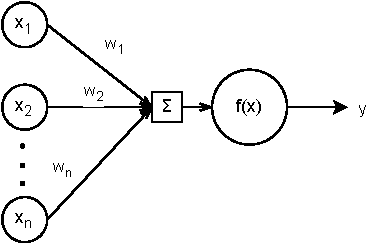
\includegraphics[width=0.5\textwidth]{images/neuron}
    \begin{itemize}
        \item[] $\Sigma$: sumator
        \item[] $f(x)$: funkcja aktywacyjna
        \item[] $w_x \  \forall x \in [1, 2, ..., n]$: wagi
        \item[] $x_x \  \forall x \in [1, 2, ..., n]$: wejścia
    \end{itemize}
    \captionsource{Schemat neuronu}{Opracowanie własne}
    \label{fig:neuron}
\end{figure}

\begin{figure}[H]
    \centering
    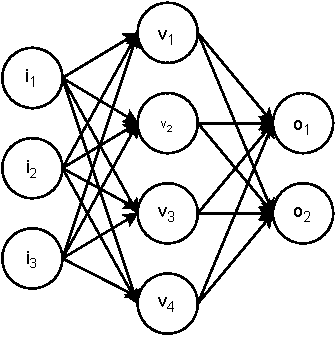
\includegraphics[width=0.5\textwidth]{images/neural-network}
    \begin{itemize}
        \item[] $i_x \ \forall x \in [1, 2, 3]$: dane wejściowe
        \item[] $v_x \ \forall x \in [1, 2, 3, 4]$: neurony w warstwie ukrytej
        \item[] $o_x \ \forall x \in [1, 2]$: dane wyjściowe
    \end{itemize}
    \captionsource{Schemat sieci neuronowej}{Opracowanie własne}
    \label{fig:neural-network}
\end{figure}
Sieci neuronowe możemy podzielić na wiele rodzajów, do których możemy zaliczyć między innymi:
\begin{itemize}
    \item \textbf{perceptron} - jest to najstarszy przykład sieci neuronowej złożonej z jednego perceptronu (neuronu).\ Można je zastosować w problemach klasyfikacji;
    \item \textbf{sieci wielowarstwowe perceptronowe} - jest to sieć złożona z wielu warstw połączonych ze sobą neuronów, najprostszy model sieci zaprezentowany na \refsource{rysunku}{fig:neural-network}.\ Składa się z warstwy wejściowej, warstw (jednej bądź wielu) ukrytych oraz warstwy wyjściowej.\ W neurony w tej sieci w porównaniu do perceptronów, mają funkcję aktywacyjną sigmoidalną, ze względu na rozwiązywanie problemów nieliniowych (posiadających więcej rozwiązań niż dwa 0/1).\ Można je zastosować na przykład do klasyfikacji danych;
    \item \textbf{sieci konwolucyjne (CNN)} - są to sieci służące do rozpoznawania obrazów, nazwa wzięła się od wykonywanej na obrazie operacji konwolucji (splotu).\ Sieci te posiadają dodatkowe warstwy konwolucyjne oraz spłaszczania, które pozwalają zamienić reprezentację obrazu w pojedyncze wartości;
    \item \textbf{sieci rekurencyjne} - charakteryzują się pętlą zwrotną w warstwie ukrytej.\ Mogą być wykorzystane do generowania tekstu, tłumaczen maszynowych, a także na przykład przewidywania cen rynkowych;
    \item \textbf{sieci samoorganizujące się} - wykorzystuje uczenie nienadzorowane oraz.\ Składają sie jedynie z warstwy wejściowej i wyjściowej.\ Zaś cechą charakterystyczną jest to, że neurony określające podobne klasy znajdują się obok siebie.\ Sieci te mogą być wykorzystywane do podziału klientów na odpowiednie grupy bądź do wskazania, jakim klientom zaproponować karty kredytowe~\cite{IBMNetwork, BartosSOM}.
\end{itemize}

\section{Głębokie uczenie}
Jest to podkategoria uczenia maszynowego polegająca na tworzeniu wielowarstwowych sieci neuronowych.\ W porównaniu do podstawowych sieci neuronowych potrzebuje ogromnych zbiorów danych do utworzenia modelu predykcyjnego.\ Potrzebuje również dużo więcej mocy obliczeniowej przez wzgląd na ilość warstw ukrytych, których może być dużo więcej, przykładem najprostszej sieci głębokiej jest \refsource{rysunek}{fig:deep-learn}.

\begin{figure}[H]
    \centering
    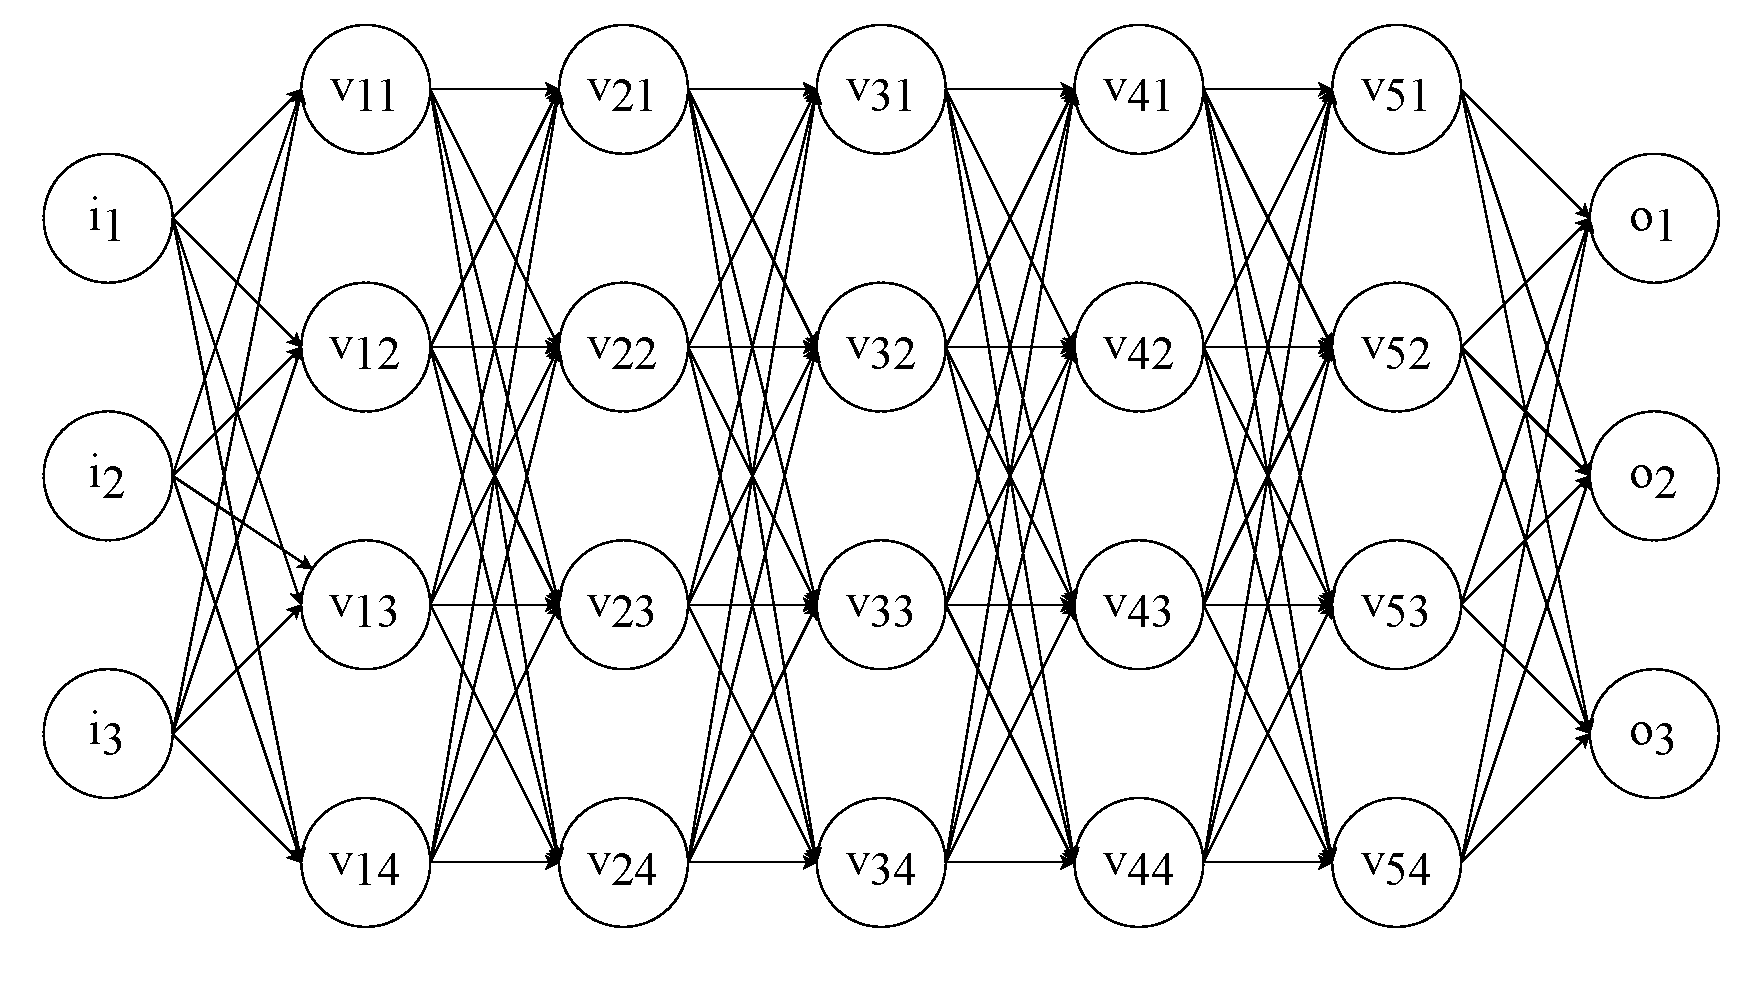
\includegraphics[width=0.5\textwidth]{images/deep-neural-network}
    \begin{itemize}
        \item[] $i_x \  \forall x \in [1, 2, 3]$: dane wejściowe
        \item[] $v_x \ \forall x \in [11, 12, 13, 21, 22, 23, 31, 32, 33]$: neurony w warstwie ukrytej
        \item[] $o_x \ \forall x \in [1, 2]$: dane wyjściowe
    \end{itemize}
    \captionsource{Schemat prostej głębokiej sieci neuronowej}{Opracowanie własne}
    \label{fig:deep-learn}
\end{figure}

Warstwa wyjściowa DNN może dostarczać dane różnego formatu, może to być na przykłąd, tekst, liczba bądź dźwięk.\ Posiada również bardzo dużo zastosowań, w których skład wchodzi generowanie treści, Deepfake, analiza obrazów, wskazywanie obiektów na obrazach, projektowanie leków, czatboty.\ Jest to udoskonalenie podstawowych sieci neuronowych.\ Tak więc część typów sieci opisanych w \refsource{sekcji}{sec:snn} będzie odnosić się do głębokich sieci neuronowych, należy do nich CNN~\cite{MicrosoftDeep2023}.